\adparagraph{Kendall Tau Distance}

\begin{figure}[H]
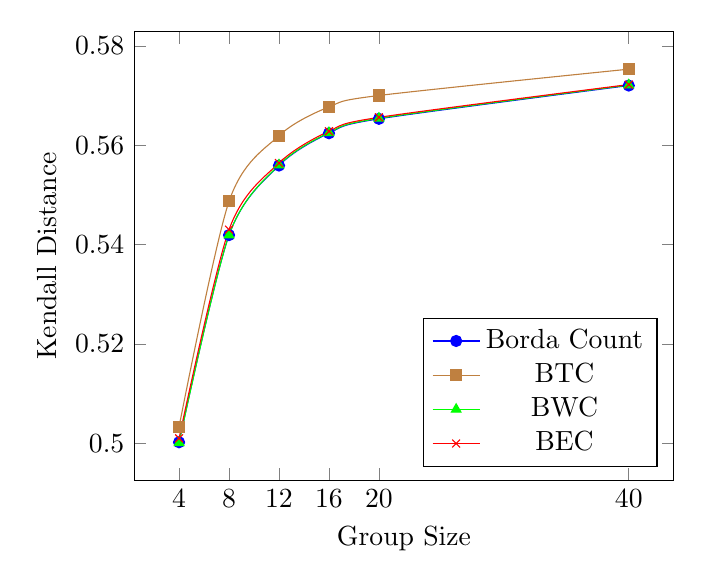
\begin{tikzpicture}
\begin{axis}[
        xlabel=Group Size,
        ylabel=Kendall Distance,
        xtick = {4,8,12,16,20,40},
        legend pos=south east]
	\addplot[smooth,mark=*,blue] plot coordinates {
        (4,0.5002)
        (8,0.5419)
        (12,0.5559)
        (16,0.5624)
        (20,0.5653)
        (40,0.572)
    };
    \addlegendentry{Borda Count}	
	
	    \addplot[smooth,color=brown,mark=square*] plot coordinates {
		(4,0.5033)
		(8,0.5487)
		(12,0.5619)
		(16,0.5677)
		(20,0.57)
		(40,0.5753)
	};
	\addlegendentry{BTC}
	
	
	\addplot[smooth,color=green,mark=triangle*] plot coordinates {
		(4,0.5001)
		(8,0.5419)
		(12,0.556)
		(16,0.5625)
		(20,0.5654)
		(40,0.5721)
	};
	\addlegendentry{BWC}
	
	
	\addplot[smooth,color=red,mark=x] plot coordinates {
		(4,0.501)
		(8,0.543)
		(12,0.5564)
		(16,0.5628)
		(20,0.5656)
		(40,0.5722)
	};
	\addlegendentry{BEC}
	
\end{axis}
\end{tikzpicture}
\caption{Results on Kendall Tau distance test for Borda Count extensions}
\end{figure}